% Designed Companion Part IV figure
% Intended for \input{...} beside the matching canonical problem.
\begin{figure}[ht]
\centering
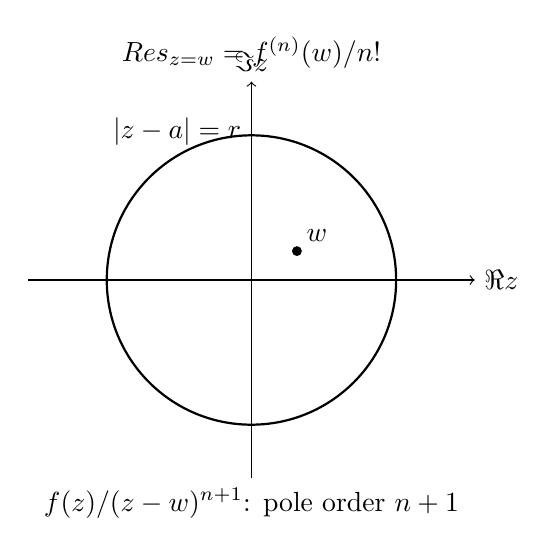
\begin{tikzpicture}[scale=1.05]
  \draw[->] (-2.7,0)--(2.7,0) node[right] {$\Re z$};
  \draw[->] (0,-2.4)--(0,2.4) node[above] {$\Im z$};
  \draw[thick,->] (0,0) circle (1.75);
  \fill (0.55,0.35) circle (1.7pt) node[above right] {$w$};
  \node at (-0.9,1.8) {$|z-a|=r$};
  \node at (0,-2.7) {$f(z)/(z-w)^{n+1}$: pole order $n+1$};
  \node at (0,2.75) {$\operatorname{Res}_{z=w}=f^{(n)}(w)/n!$};
\end{tikzpicture}
\caption{The integrand $f(z)/(z-w)^{n+1}$ has a single higher-order pole at $w$ inside the contour. Its residue is $f^{(n)}(w)/n!$, which is exactly the coefficient extracted by Cauchy's derivative formula.}
\label{fig:cp-iv-0139-higher-order-pole-cauchy}
\end{figure}
